%%%%%%%%%%%%%%%%%%%%%%%%%%%%%%%%%%%%%%%%%%%%%%%%%%%%%%%%%%%%%%%%%%%%%%
% Slides
%%%%%%%%%%%%%%%%%%%%%%%%%%%%%%%%%%%%%%%%%%%%%%%%%%%%%%%%%%%%%%%%%%%%%%

\begin{frame}
\titlepage
\end{frame}

\begin{frame}{Sumário}
  \tableofcontents
\end{frame}

\section{Introdução}

%\section{Problema}
\begin{frame}{Problema}
	No sistema de arquivos distribuído, o método de replicação de arquivos é muito prático e eficiente para tolerar as falhas sobre dados, porém consome muito espaço no dispositivo de armazenamento. Quando ocorre a falta de espaço, novos servidores vão ser adicionados no conjunto para incrementar a capacidade de armazenamento do sistema. Isso gera o custo de de implantação de equipamentos, além de causar o aumento no custo de manutenção permanente do sistema.
\end{frame} 

\section{Diretriz da pesquisa}
\begin{frame}{Objetivo e Hipótese}
	
	\begin{block}{Objetivo}
		Construir um sistema de arquivos distribuído que armazena os dados de forma mais eficiente que o método de replicação, evitando o aumento do custo de manutenção por incremento de escala do sistema.
		
	\end{block}
	
	\begin{block}{Hipótese}
		O conceito de RAID pode oferecer a proteção de arquivos para sistema consumindo menos espaço que a replicação, apresentando menos espaço ocupado pela parte redundante dos arquivos. 
		
	\end{block}
	
\end{frame}

\begin{frame}{Metodologia}
	
	\begin{block}{Estudos bibliográficos}
		\begin{itemize}
			\item Conceitos de proteção de dados da tecnologia RAID.
			\item Arquitetura do sistema de arquivos distribuídos.
		\end{itemize}
	\end{block}
	
	\begin{block}{Elaboração e implementaçao do sistema}
		
	\end{block}
	
	\begin{block}{Coleta de dados por execução do sistema}
		
	\end{block}
	
	\begin{block}{Análise de dados}
		\begin{itemize}
			\item Comparação entre os métodos de replicação e RAID.
		\end{itemize}
		
	\end{block}
	
\end{frame}

\section{Fundamentação teórica}

\begin{frame}{Sistema de arquivos distribuído}
	%\textbf{Sistema de arquivos distribuído}
	\begin{itemize}
		\item Conjunto de vários servidores distribuídos fisicamente, conectados através de redes locais ou internet.
		\item Voltado para gerenciamento e armazenamento de arquivos em larga escala.
		\item Cria algumas copias de segurança dos dados, chamadas de réplicas, cujas são armazenadas espalhadamente entre os servidores.
		%\item 	
	\end{itemize}
\end{frame}

\begin{frame}{}
	\begin{columns}
		\column{0.5\textwidth}
		Réplica:
		\begin{itemize}
			\item Tolera as falhas que impedem o acesso aos arquivos armazenados,
			\item Distribui as cargas de acesso entre servidores.
		\end{itemize}
		
		\column{0.5\textwidth}
		\begin{figure}
			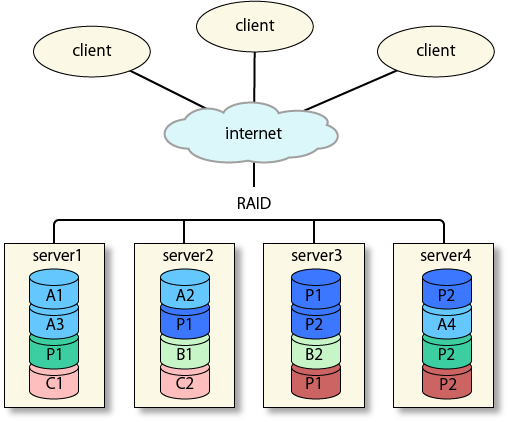
\includegraphics[width=\textwidth]{image1}
			\label{fig:exemplo}
		\end{figure}
		
		
		%\column{0.25\textwidth}
	\end{columns}
\end{frame}

\begin{frame}{}
	\begin{columns}
		\column{0.45\textwidth}
		
		\begin{figure}
			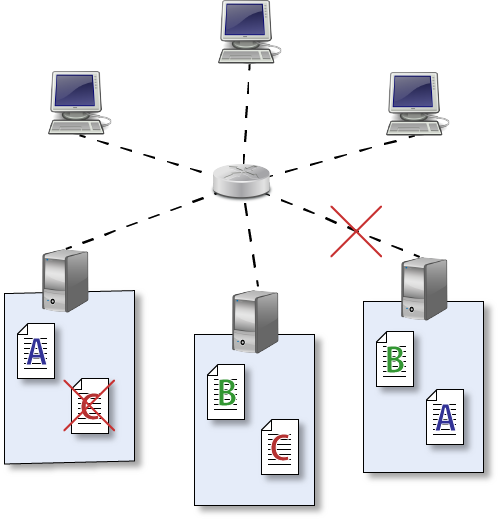
\includegraphics[width=\textwidth]{image2}
			\caption{Tolerância a falha}
			\label{fig:exemplo}
		\end{figure}
		
		\column{0.1\textwidth}
		
		\column{0.45\textwidth}
		
		\begin{figure}
			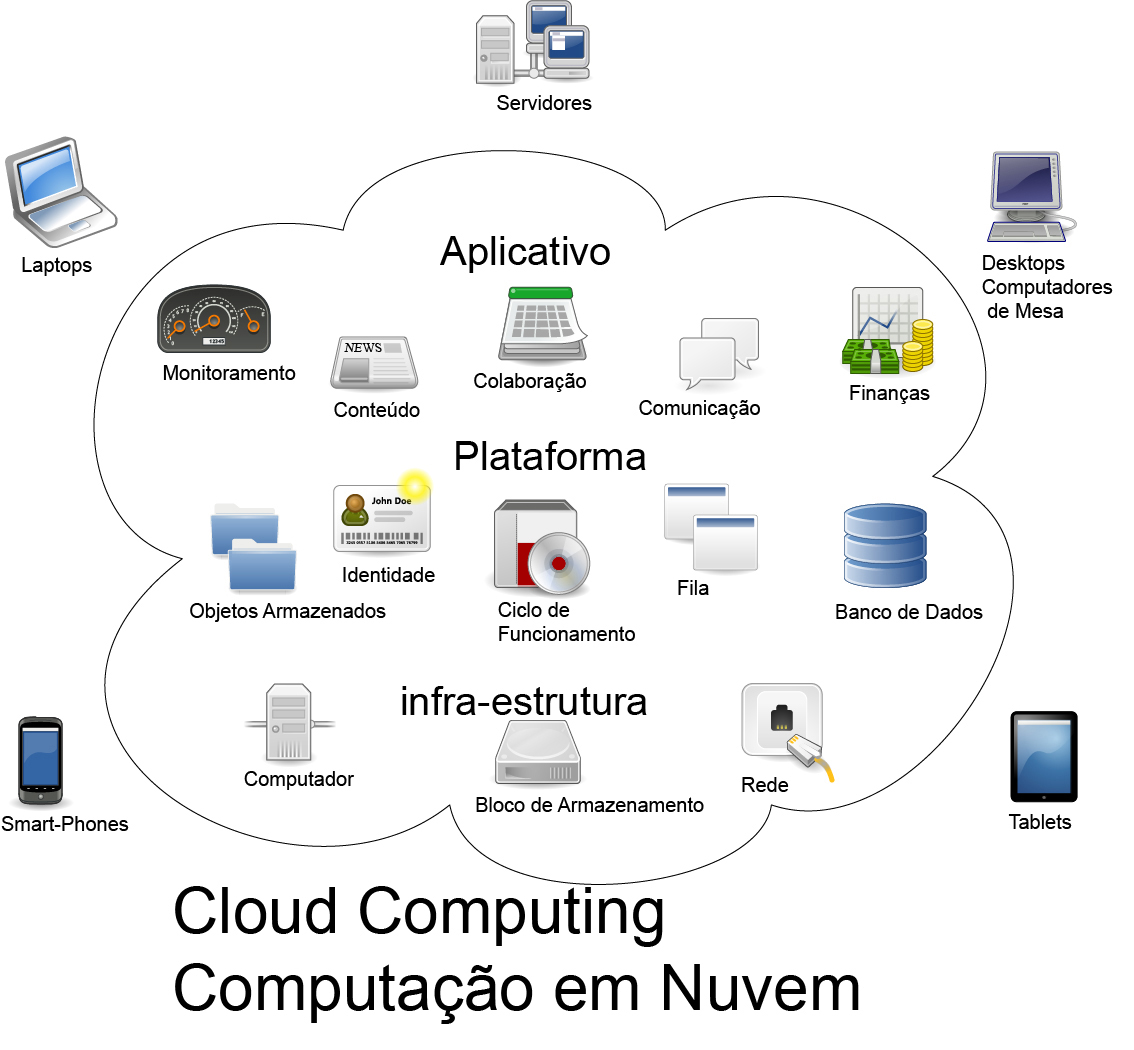
\includegraphics[width=\textwidth]{image3}
			\caption{Distribuição da carga}
			\label{fig:exemplo}
		\end{figure}
		
		
		%\column{0.25\textwidth}
	\end{columns}
\end{frame}
\begin{frame}{RAID}
	
	\begin{itemize}
		\item \textit{Redundant Array of Independent Disks}.
		\item Trata-se, basicamente, de uma solução computacional que combina vários discos rígidos (HDs) para formar uma única unidade lógica de armazenamento de dados.
		\item Vantagens:
		\begin{itemize}
			\item Se um HD sofrer danos, os dados existentes nele não serão perdidos, pois podem ser replicados em outra unidade (redundância).
			\item É possível aumentar a capacidade de armazenamento a qualquer momento com a adição de mais HDs.
			\item O acesso à informação pode se tornar mais rápido, pois os dados são distribuídos a todos os discos.
			\item Dependendo do caso, há maior tolerância a falhas, pois o sistema não é paralisado se uma unidade parar de funcionar.
		\end{itemize}
	\end{itemize}
\end{frame}

\begin{frame}{RAID}
	\begin{itemize}
		\item Níveis de RAID
		\begin{itemize}
			\item RAID 0
			\item RAID 1
			\item RAID 5
			\item RAID 50
		\end{itemize}
	\end{itemize}
\end{frame}

\begin{frame}{RAID 0}
	\begin{columns}
		\column{0.5\textwidth}
		\begin{itemize}
			\item Striping (fracionamento).
			\item Não oferece proteção contra falhas, pois não existe redundância.
			\item Focado no desempenho. Visto que quanto mais discos houver no sistema, maior é a sua taxa de transferência devido ao paralelismo nas operações de leitura e escrita.
		\end{itemize}
		
		\column{0.25\textwidth}
		\begin{figure}
			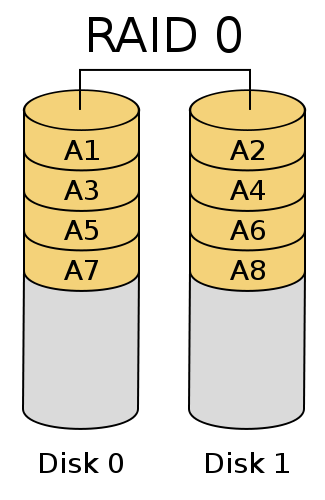
\includegraphics[width=\textwidth]{RAID_0}
			\label{fig:exemplo}
		\end{figure}
		
	\end{columns}
\end{frame}

\begin{frame}{RAID 1}
	\begin{columns}
		\column{0.5\textwidth}
		\begin{itemize}
			\item Mirror (Espelhamento).
			\item Necessita de uma quantidade par de discos.
			\item Vantagem
			\begin{itemize}
				\item Evita falhas físicas.
			\end{itemize}
			\item Desvantagens
			\begin{itemize}
				\item Perda de desempenho.
				\item Alto desperdício de espaço.
				\item  Não dispensa soluções de \textit{backup}.
			\end{itemize}
		\end{itemize}
		
		\column{0.25\textwidth}
		\begin{figure}
			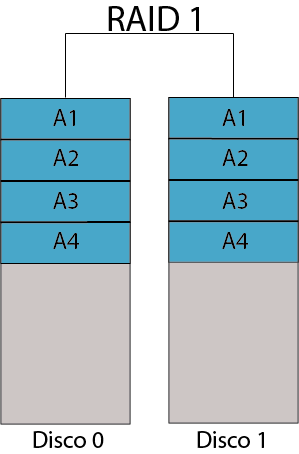
\includegraphics[width=\textwidth]{RAID_1}
			\label{fig:exemplo}
		\end{figure}
		
	\end{columns}
\end{frame}


\begin{frame}{RAID 5}
	\begin{columns}
		\column{0.5\textwidth}
		\begin{itemize}
			\item Esquema de paridade, pelo uso do bit de paridade.
			\item A informação sobre paridade é distribuída entre todos os discos.
			\item Vantagens
			\begin{itemize}
				\item Tolerância a falhas.
				\item Leitura rápida.
			\end{itemize}
			\item Desvantagens
			\begin{itemize}
				\item Sistema complexo de controle dos discos.
			\end{itemize}
		\end{itemize}
		
		\column{0.5\textwidth}
		\begin{figure}
			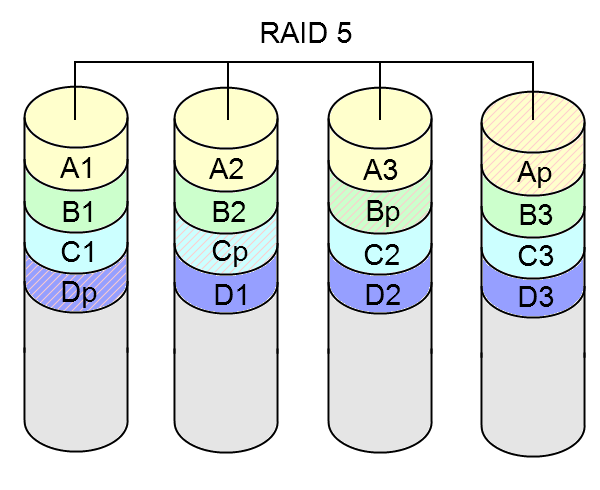
\includegraphics[width=\textwidth]{RAID_5}
			\label{fig:exemplo}
		\end{figure}
		
	\end{columns}
\end{frame}

\begin{frame}{RAID 50}
	\begin{columns}
		\column{0.5\textwidth}
		\begin{itemize}
			\item Paridade em conjunção com a segmentação de dados.
			\item Vantagens
			\begin{itemize}
				\item Tolerância a falhas.
				\item Alta taxa de transferência de dados.
			\end{itemize}
			\item Desvantagens
			\begin{itemize}
				\item Sistema ainda mais complexo de controle dos discos.
			\end{itemize}
		\end{itemize}
		
		\column{0.5\textwidth}
		\begin{figure}
			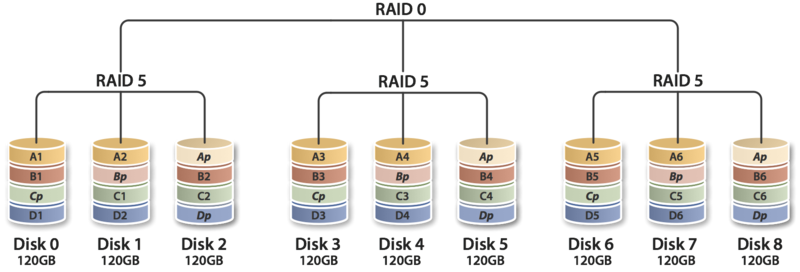
\includegraphics[width=\textwidth]{RAID_50}
			\label{fig:exemplo}
		\end{figure}
		
	\end{columns}
\end{frame}

\section{Sistema proposto}
\begin{frame}{Sistema de arquivo distribuído com RAID}
	
	\begin{columns}
		\column{0.5\textwidth}
		\begin{itemize}
			\item Os arquivos são divididos em vários blocos.
			\item Gera a paridade para grupo de alguns blocos.
			\item Armazena distribuidamente por servidores.
			\item Fornece tolerância a falha e distribuição de carga com menos espaço usado por parte redundante.
		\end{itemize}
		\column{0.5\textwidth}
		
		\begin{figure}
			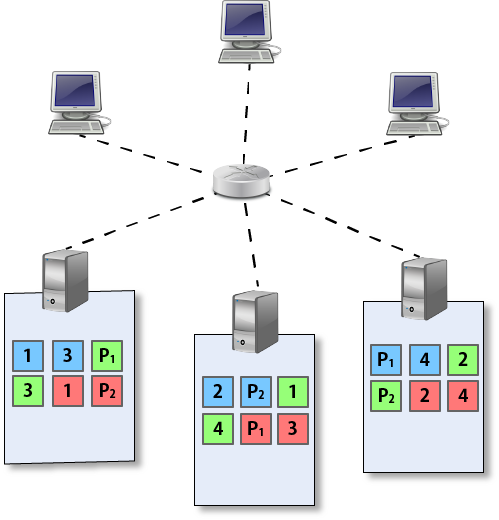
\includegraphics[width=\textwidth]{image4}
			%\caption{}
			\label{fig:exemplo}
		\end{figure}
	\end{columns}
	
\end{frame}


\begin{frame}{}
	
	\begin{figure}
		\includegraphics[width=\textwidth]{image5}
		\caption{Geração de paridade e recuperação de arquivo}
		\label{fig:exemplo}
	\end{figure}
	
\end{frame}

\section{Bibliografia}
\begin{frame}{Bibliografia}
	\begin{itemize}
		\item Andrew S. Tanenbaum and M. van Steen. Distributed Systems: Principles and Paradigms. Pearson Prentice Hall, 2007.
		\item Berislav Biocié Drasko Tomié and Osman Muftié. A novel scheduling approach of elearning content on cloud computing infrastructure. MIPRO, 2011.
		\item Eliezer Levy and Abraham Silberschatz. Distributed file systems: Concepts and examples. ACM Computing Surveys, 1990.
		\item David A. Patterson and Garth Gibson and Randy H. Katz. A case for redundant arrays
		of inexpensive disks (RAID). SIGMOD Rec, 1988.
	\end{itemize}
\end{frame}

\section{}
\begin{frame}
	\frametitle{Obrigado pela atenção!}
	\begin{center}
		{\Huge Obrigado!}
	\end{center}
\end{frame}
